% Options for packages loaded elsewhere
\PassOptionsToPackage{unicode}{hyperref}
\PassOptionsToPackage{hyphens}{url}
\documentclass[
]{article}
\usepackage{xcolor}
\usepackage[margin=1in]{geometry}
\usepackage{amsmath,amssymb}
\setcounter{secnumdepth}{5}
\usepackage{iftex}
\ifPDFTeX
  \usepackage[T1]{fontenc}
  \usepackage[utf8]{inputenc}
  \usepackage{textcomp} % provide euro and other symbols
\else % if luatex or xetex
  \usepackage{unicode-math} % this also loads fontspec
  \defaultfontfeatures{Scale=MatchLowercase}
  \defaultfontfeatures[\rmfamily]{Ligatures=TeX,Scale=1}
\fi
\usepackage{lmodern}
\ifPDFTeX\else
  % xetex/luatex font selection
\fi
% Use upquote if available, for straight quotes in verbatim environments
\IfFileExists{upquote.sty}{\usepackage{upquote}}{}
\IfFileExists{microtype.sty}{% use microtype if available
  \usepackage[]{microtype}
  \UseMicrotypeSet[protrusion]{basicmath} % disable protrusion for tt fonts
}{}
\makeatletter
\@ifundefined{KOMAClassName}{% if non-KOMA class
  \IfFileExists{parskip.sty}{%
    \usepackage{parskip}
  }{% else
    \setlength{\parindent}{0pt}
    \setlength{\parskip}{6pt plus 2pt minus 1pt}}
}{% if KOMA class
  \KOMAoptions{parskip=half}}
\makeatother
\usepackage{color}
\usepackage{fancyvrb}
\newcommand{\VerbBar}{|}
\newcommand{\VERB}{\Verb[commandchars=\\\{\}]}
\DefineVerbatimEnvironment{Highlighting}{Verbatim}{commandchars=\\\{\}}
% Add ',fontsize=\small' for more characters per line
\usepackage{framed}
\definecolor{shadecolor}{RGB}{248,248,248}
\newenvironment{Shaded}{\begin{snugshade}}{\end{snugshade}}
\newcommand{\AlertTok}[1]{\textcolor[rgb]{0.94,0.16,0.16}{#1}}
\newcommand{\AnnotationTok}[1]{\textcolor[rgb]{0.56,0.35,0.01}{\textbf{\textit{#1}}}}
\newcommand{\AttributeTok}[1]{\textcolor[rgb]{0.13,0.29,0.53}{#1}}
\newcommand{\BaseNTok}[1]{\textcolor[rgb]{0.00,0.00,0.81}{#1}}
\newcommand{\BuiltInTok}[1]{#1}
\newcommand{\CharTok}[1]{\textcolor[rgb]{0.31,0.60,0.02}{#1}}
\newcommand{\CommentTok}[1]{\textcolor[rgb]{0.56,0.35,0.01}{\textit{#1}}}
\newcommand{\CommentVarTok}[1]{\textcolor[rgb]{0.56,0.35,0.01}{\textbf{\textit{#1}}}}
\newcommand{\ConstantTok}[1]{\textcolor[rgb]{0.56,0.35,0.01}{#1}}
\newcommand{\ControlFlowTok}[1]{\textcolor[rgb]{0.13,0.29,0.53}{\textbf{#1}}}
\newcommand{\DataTypeTok}[1]{\textcolor[rgb]{0.13,0.29,0.53}{#1}}
\newcommand{\DecValTok}[1]{\textcolor[rgb]{0.00,0.00,0.81}{#1}}
\newcommand{\DocumentationTok}[1]{\textcolor[rgb]{0.56,0.35,0.01}{\textbf{\textit{#1}}}}
\newcommand{\ErrorTok}[1]{\textcolor[rgb]{0.64,0.00,0.00}{\textbf{#1}}}
\newcommand{\ExtensionTok}[1]{#1}
\newcommand{\FloatTok}[1]{\textcolor[rgb]{0.00,0.00,0.81}{#1}}
\newcommand{\FunctionTok}[1]{\textcolor[rgb]{0.13,0.29,0.53}{\textbf{#1}}}
\newcommand{\ImportTok}[1]{#1}
\newcommand{\InformationTok}[1]{\textcolor[rgb]{0.56,0.35,0.01}{\textbf{\textit{#1}}}}
\newcommand{\KeywordTok}[1]{\textcolor[rgb]{0.13,0.29,0.53}{\textbf{#1}}}
\newcommand{\NormalTok}[1]{#1}
\newcommand{\OperatorTok}[1]{\textcolor[rgb]{0.81,0.36,0.00}{\textbf{#1}}}
\newcommand{\OtherTok}[1]{\textcolor[rgb]{0.56,0.35,0.01}{#1}}
\newcommand{\PreprocessorTok}[1]{\textcolor[rgb]{0.56,0.35,0.01}{\textit{#1}}}
\newcommand{\RegionMarkerTok}[1]{#1}
\newcommand{\SpecialCharTok}[1]{\textcolor[rgb]{0.81,0.36,0.00}{\textbf{#1}}}
\newcommand{\SpecialStringTok}[1]{\textcolor[rgb]{0.31,0.60,0.02}{#1}}
\newcommand{\StringTok}[1]{\textcolor[rgb]{0.31,0.60,0.02}{#1}}
\newcommand{\VariableTok}[1]{\textcolor[rgb]{0.00,0.00,0.00}{#1}}
\newcommand{\VerbatimStringTok}[1]{\textcolor[rgb]{0.31,0.60,0.02}{#1}}
\newcommand{\WarningTok}[1]{\textcolor[rgb]{0.56,0.35,0.01}{\textbf{\textit{#1}}}}
\usepackage{graphicx}
\makeatletter
\newsavebox\pandoc@box
\newcommand*\pandocbounded[1]{% scales image to fit in text height/width
  \sbox\pandoc@box{#1}%
  \Gscale@div\@tempa{\textheight}{\dimexpr\ht\pandoc@box+\dp\pandoc@box\relax}%
  \Gscale@div\@tempb{\linewidth}{\wd\pandoc@box}%
  \ifdim\@tempb\p@<\@tempa\p@\let\@tempa\@tempb\fi% select the smaller of both
  \ifdim\@tempa\p@<\p@\scalebox{\@tempa}{\usebox\pandoc@box}%
  \else\usebox{\pandoc@box}%
  \fi%
}
% Set default figure placement to htbp
\def\fps@figure{htbp}
\makeatother
\setlength{\emergencystretch}{3em} % prevent overfull lines
\providecommand{\tightlist}{%
  \setlength{\itemsep}{0pt}\setlength{\parskip}{0pt}}
\usepackage[]{natbib}
\bibliographystyle{plainnat}
\usepackage{bookmark}
\IfFileExists{xurl.sty}{\usepackage{xurl}}{} % add URL line breaks if available
\urlstyle{same}
\hypersetup{
  pdftitle={HW 06 - Money in US politics},
  hidelinks,
  pdfcreator={LaTeX via pandoc}}

\title{HW 06 - Money in US politics}
\author{}
\date{\vspace{-2.5em}}

\begin{document}
\maketitle

{
\setcounter{tocdepth}{2}
\tableofcontents
}
\begin{figure}
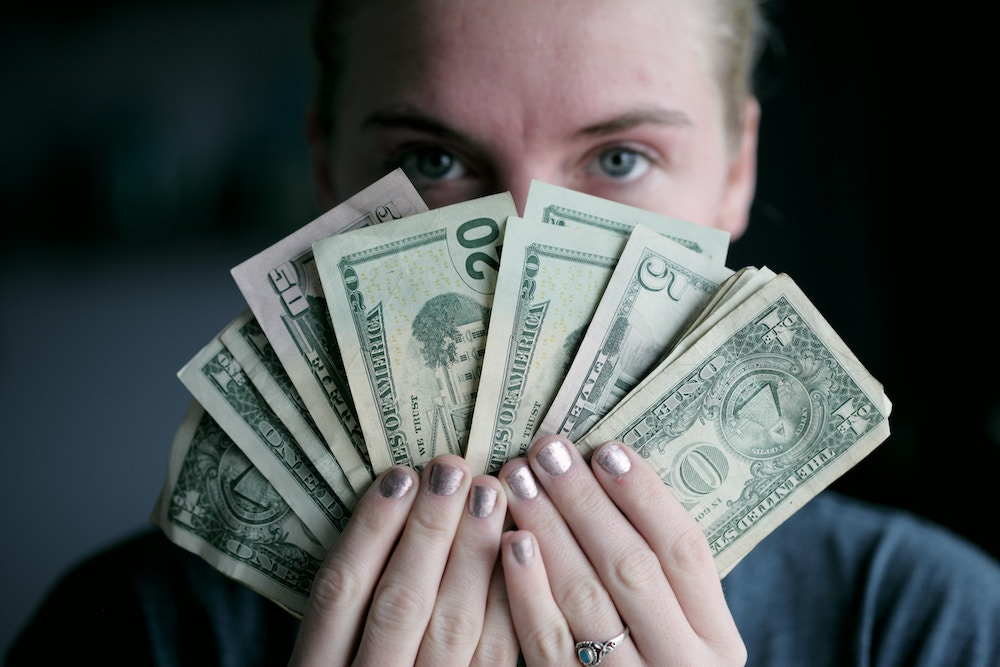
\includegraphics[width=0.8\linewidth]{img/sharon-mccutcheon-rItGZ4vquWk-unsplash} \caption{Photo by Sharon McCutcheon on Unsplash}\label{fig:photo}
\end{figure}

Every election cycle brings its own brand of excitement -- and lots of
money. Political donations are of particular interest to political
scientists and other researchers studying politics and voting patterns.
They are also of interest to citizens who want to stay informed of how
much money their candidates raise and where that money comes from.

In the United States, \emph{``only American citizens (and immigrants
with green cards) can contribute to federal politics, but the American
divisions of foreign companies can form political action committees
(PACs) and collect contributions from their American
employees.''}\footnote{Source:
  \href{https://www.opensecrets.org/political-action-committees-pacs/foreign-connected-pacs}{Open
  Secrets - Foreign Connected PACs}.}

In this assignment we will scrape and work with data foreign connected
PACs that donate to US political campaigns. First, we will get data
foreign connected PAC contributions in the 2022 election cycle. Then,
you will use a similar approach to get data such contributions from
previous years so that we can examine trends over time.

In order to complete this assignment you will need a Chrome browser with
the \href{http://selectorgadget.com/}{Selector Gadget extension}
installed.

\section{Getting started}\label{getting-started}

Go to the course GitHub organization and locate your homework repo,
clone it in RStudio and open the R Markdown document. Knit the document
to make sure it compiles without errors.

\subsection{Warm up}\label{warm-up}

Before we introduce the data, let's warm up with some simple exercises.
Update the YAML of your R Markdown file with your information, knit,
commit, and push your changes. Make sure to commit with a meaningful
commit message. Then, go to your repo on GitHub and confirm that your
changes are visible in your Rmd \textbf{and} md files. If anything is
missing, commit and push again.

\subsection{Packages}\label{packages}

We'll use the \textbf{tidyverse} package for much of the data wrangling
and visualisation, the \textbf{robotstxt} package to check if we're
allowed to scrape the data, the \textbf{rvest} package for data
scraping, and the \textbf{scales} package for better formatting of
labels on visualisations. These packages are already installed for you.
You can load them by running the following in your Console:

\begin{Shaded}
\begin{Highlighting}[]
\FunctionTok{library}\NormalTok{(tidyverse)}
\FunctionTok{library}\NormalTok{(robotstxt)}
\FunctionTok{library}\NormalTok{(rvest)}
\FunctionTok{library}\NormalTok{(scales)}
\end{Highlighting}
\end{Shaded}

\subsection{Data}\label{data}

This assignment does not come with any prepared datasets. Instead you'll
be scraping the data!

\section{Exercises}\label{exercises}

\subsection{Data collection via web
scraping}\label{data-collection-via-web-scraping}


\includegraphics[width=0.8\linewidth]{img/opensecrets}

The data come from \href{https://www.opensecrets.org}{OpenSecrets.org},
a \emph{``website tracking the influence of money on U.S. politics, and
how that money affects policy and citizens' lives''}. This website is
hosted by The Center for Responsive Politics, which is a nonpartisan,
independent nonprofit that \emph{``tracks money in U.S. politics and its
effect on elections and public policy.''}\footnote{Source:
  \href{https://www.opensecrets.org/about/}{Open Secrets - About}.}

Before getting started, let's check that a bot has permissions to access
pages on this domain.

\begin{Shaded}
\begin{Highlighting}[]
\FunctionTok{library}\NormalTok{(robotstxt)}
\FunctionTok{paths\_allowed}\NormalTok{(}\StringTok{"https://www.opensecrets.org"}\NormalTok{)}
\end{Highlighting}
\end{Shaded}

\begin{verbatim}
## [1] TRUE
\end{verbatim}

Our goal is to scrape data for contributions in all election years Open
Secrets has data for. Since that means repeating a task many times,
let's first write a function that works on the first page. Confirm it
works on a few others. Then iterate it over pages for all years.

Complete the following set of steps in the \texttt{scrape-pac.R} file in
the \texttt{scripts} folder of your repository. This file already
contains some starter code to help you out.

\begin{itemize}
\item
  Write a function called \texttt{scrape\_pac()} that scrapes
  information from the Open Secrets webpage for foreign-connected PAC
  contributions in a given year. This function should

  \begin{itemize}
  \tightlist
  \item
    have one input: the URL of the webpage and should return a data
    frame.
  \item
    rename variables scraped, using \texttt{snake\_case} naming.
  \item
    clean up the \texttt{Country\ of\ Origin/Parent\ Company} variable
    with \texttt{str\_squish()}.
  \item
    add a new column to the data frame for \texttt{year}. We will want
    this information when we ultimately have data from all years, so
    this is a good time to keep track of it. Our function doesn't take a
    year argument, but the year is embedded in the URL, so we can
    extract it out of there, and add it as a new column. Use the
    \texttt{str\_sub()} function to extract the last 4 characters from
    the URL. You will probably want to look at the help for this
    function to figure out how to specify ``last 4 characters''.
  \end{itemize}
\item
  Define the URLs for 2022, 2020, and 2000 contributions. Then, test
  your function using these URLs as inputs. Does the function seem to do
  what you expected it to do?
\item
  Construct a vector called \texttt{urls} that contains the URLs for
  each webpage that contains information on foreign-connected PAC
  contributions for a given year.
\item
  Map the \texttt{scrape\_pac()} function over \texttt{urls} in a way
  that will result in a data frame called \texttt{pac\_all}.
\item
  Write the data frame to a csv file called \texttt{pac-all.csv} in the
  \texttt{data} folder.
\end{itemize}

\emph{If you haven't yet done so, now is definitely a good time to
commit and push your changes to GitHub with an appropriate commit
message (e.g.~``Data scraping complete''). Make sure to commit and push
all changed files so that your Git pane is cleared up afterwards.}

Complete the following set of steps in the \texttt{hw-06.Rmd} file in
your repository.

\begin{enumerate}
\def\labelenumi{\arabic{enumi}.}
\tightlist
\item
  In your R Markdown file, load \texttt{pac-all.csv} and report its
  number of observations and variables using inline code.
\end{enumerate}

\begin{Shaded}
\begin{Highlighting}[]
\CommentTok{\# Load the scraped data}
\NormalTok{pac\_all }\OtherTok{\textless{}{-}} \FunctionTok{read\_csv}\NormalTok{(}\StringTok{"data/pac{-}all.csv"}\NormalTok{)}
\end{Highlighting}
\end{Shaded}

\begin{verbatim}
## Rows: 2404 Columns: 6
## -- Column specification --------------------------------------------------------
## Delimiter: ","
## chr (5): name, country_parent, total, dems, repubs
## dbl (1): year
## 
## i Use `spec()` to retrieve the full column specification for this data.
## i Specify the column types or set `show_col_types = FALSE` to quiet this message.
\end{verbatim}

The dataset contains 2404 observations and 6 variables.

\subsection{Data cleaning}\label{data-cleaning}

In this section we clean the \texttt{pac\_all} data frame to prepare it
for analysis and visualization. We have two goals in data cleaning:

\begin{itemize}
\item
  Separate the \texttt{country\_parent} into two such that country and
  parent company appear in different columns for country-level analysis.
\item
  Convert contribution amounts in \texttt{total}, \texttt{dems}, and
  \texttt{repubs} from character strings to numeric values.
\end{itemize}

The following exercises walk you through how to make these fixes to the
data.

\begin{enumerate}
\def\labelenumi{\arabic{enumi}.}
\setcounter{enumi}{1}
\tightlist
\item
  Use the \texttt{separate()} function to separate
  \texttt{country\_parent} into \texttt{country} and \texttt{parent}
  columns. Note that country and parent company names are separated by
  \texttt{\textbackslash{}} (which will need to be specified in your
  function) and also note that there are some entries where the
  \texttt{\textbackslash{}} sign appears twice and in these cases we
  want to only split the value at the first occurrence of
  \texttt{\textbackslash{}}. This can be accomplished by setting the
  \texttt{extra} argument in to \texttt{"merge"} so that the cell is
  split into only 2 segments, e.g.~we want
  \texttt{"Denmark/Novo\ Nordisk\ A/S"} to be split into
  \texttt{"Denmark"} and \texttt{"Novo\ Nordisk\ A/S"}. (See help for
  \texttt{separate()} for more on this.) End your code chunk by printing
  out the top 10 rows of your data frame (if you just type the data
  frame name it should automatically do this for you).
\end{enumerate}

\begin{Shaded}
\begin{Highlighting}[]
\CommentTok{\# Separate country\_parent into country and parent columns}
\NormalTok{pac\_all }\OtherTok{\textless{}{-}}\NormalTok{ pac\_all }\SpecialCharTok{\%\textgreater{}\%}
  \FunctionTok{separate}\NormalTok{(country\_parent, }\AttributeTok{into =} \FunctionTok{c}\NormalTok{(}\StringTok{"country"}\NormalTok{, }\StringTok{"parent"}\NormalTok{), }\AttributeTok{sep =} \StringTok{"/"}\NormalTok{, }\AttributeTok{extra =} \StringTok{"merge"}\NormalTok{)}

\CommentTok{\# Print top 10 rows}
\NormalTok{pac\_all}
\end{Highlighting}
\end{Shaded}

\begin{verbatim}
## # A tibble: 2,404 x 7
##    name                                  country parent total dems  repubs  year
##    <chr>                                 <chr>   <chr>  <chr> <chr> <chr>  <dbl>
##  1 7-Eleven                              Japan   Ito-Y~ $8,5~ $1,5~ $7,000  2000
##  2 ABB Group                             Switze~ Asea ~ $46,~ $17,~ $28,5~  2000
##  3 Accenture                             UK      Accen~ $75,~ $23,~ $52,9~  2000
##  4 ACE INA                               UK      ACE G~ $38,~ $12,~ $26,0~  2000
##  5 Acuson Corp (Siemens AG)              Germany Sieme~ $2,0~ $2,0~ $0      2000
##  6 Adtranz (DaimlerChrysler)             Germany Daiml~ $10,~ $10,~ $500    2000
##  7 AE Staley Manufacturing (Tate & Lyle) UK      Tate ~ $24,~ $10,~ $14,0~  2000
##  8 AEGON USA (AEGON NV)                  Nether~ Aegon~ $58,~ $10,~ $47,7~  2000
##  9 AIM Management Group                  UK      AMVES~ $25,~ $10,~ $15,0~  2000
## 10 Air Liquide America                   France  L'Air~ $0    $0    $0      2000
## # i 2,394 more rows
\end{verbatim}

\begin{enumerate}
\def\labelenumi{\arabic{enumi}.}
\setcounter{enumi}{2}
\item
  Remove the character strings including \texttt{\$} and \texttt{,}
  signs in the \texttt{total}, \texttt{dems},and \texttt{repubs} columns
  and convert these columns to numeric. End your code chunk by printing
  out the top 10 rows of your data frame (if you just type the data
  frame name it should automatically do this for you). A couple hints to
  help you out:

  \begin{itemize}
  \item
    The \texttt{\$} character is a special character so it will need to
    be escaped.
  \item
    Some contribution amounts are in the millions (e.g.~Anheuser-Busch
    contributed a total of \$1,510,897 in 2008). In this case we need to
    remove all occurrences of \texttt{,}, which we can do by using
    \texttt{str\_remove\_all()} instead of \texttt{str\_remove()}.
  \end{itemize}
\end{enumerate}

\begin{Shaded}
\begin{Highlighting}[]
\CommentTok{\# Clean currency columns and convert to numeric}
\NormalTok{pac\_all }\OtherTok{\textless{}{-}}\NormalTok{ pac\_all }\SpecialCharTok{\%\textgreater{}\%}
  \FunctionTok{mutate}\NormalTok{(}
    \AttributeTok{total =} \FunctionTok{str\_remove\_all}\NormalTok{(total, }\StringTok{"}\SpecialCharTok{\textbackslash{}\textbackslash{}}\StringTok{$|,"}\NormalTok{) }\SpecialCharTok{\%\textgreater{}\%} \FunctionTok{as.numeric}\NormalTok{(),}
    \AttributeTok{dems =} \FunctionTok{str\_remove\_all}\NormalTok{(dems, }\StringTok{"}\SpecialCharTok{\textbackslash{}\textbackslash{}}\StringTok{$|,"}\NormalTok{) }\SpecialCharTok{\%\textgreater{}\%} \FunctionTok{as.numeric}\NormalTok{(),}
    \AttributeTok{repubs =} \FunctionTok{str\_remove\_all}\NormalTok{(repubs, }\StringTok{"}\SpecialCharTok{\textbackslash{}\textbackslash{}}\StringTok{$|,"}\NormalTok{) }\SpecialCharTok{\%\textgreater{}\%} \FunctionTok{as.numeric}\NormalTok{()}
\NormalTok{  )}

\CommentTok{\# Print top 10 rows}
\NormalTok{pac\_all}
\end{Highlighting}
\end{Shaded}

\begin{verbatim}
## # A tibble: 2,404 x 7
##    name                                  country parent total  dems repubs  year
##    <chr>                                 <chr>   <chr>  <dbl> <dbl>  <dbl> <dbl>
##  1 7-Eleven                              Japan   Ito-Y~  8500  1500   7000  2000
##  2 ABB Group                             Switze~ Asea ~ 46000 17000  28500  2000
##  3 Accenture                             UK      Accen~ 75984 23000  52984  2000
##  4 ACE INA                               UK      ACE G~ 38500 12500  26000  2000
##  5 Acuson Corp (Siemens AG)              Germany Sieme~  2000  2000      0  2000
##  6 Adtranz (DaimlerChrysler)             Germany Daiml~ 10500 10000    500  2000
##  7 AE Staley Manufacturing (Tate & Lyle) UK      Tate ~ 24000 10000  14000  2000
##  8 AEGON USA (AEGON NV)                  Nether~ Aegon~ 58250 10500  47750  2000
##  9 AIM Management Group                  UK      AMVES~ 25000 10000  15000  2000
## 10 Air Liquide America                   France  L'Air~     0     0      0  2000
## # i 2,394 more rows
\end{verbatim}

\emph{Now is a good time to knit your document, commit, and push your
changes to GitHub with an appropriate commit message. Make sure to
commit and push all changed files so that your Git pane is cleared up
afterwards.}

\subsection{Data visualization and
interpretation}\label{data-visualization-and-interpretation}

\begin{enumerate}
\def\labelenumi{\arabic{enumi}.}
\setcounter{enumi}{3}
\item
  Create a line plot of total contributions from all foreign-connected
  PACs in the Canada and Mexico over the years. Once you have made the
  plot, write a brief interpretation of what the graph reveals. Few
  hints to help you out:

  \begin{itemize}
  \tightlist
  \item
    Filter for only \texttt{Canada} and \texttt{Mexico}.
  \item
    Calculate sum of total contributions from PACs for each year for
    each country by using a sequence of \texttt{group\_by()} then
    \texttt{summarise()}.
  \item
    Make a plot of total contributions (y-axis) by year (x-axis) where
    two lines identified by different colours represent each of Canada
    and Mexico.
  \end{itemize}
\end{enumerate}

\begin{Shaded}
\begin{Highlighting}[]
\CommentTok{\# Filter for Canada and Mexico, group by year and country, then plot}
\NormalTok{pac\_all }\SpecialCharTok{\%\textgreater{}\%}
  \FunctionTok{filter}\NormalTok{(country }\SpecialCharTok{\%in\%} \FunctionTok{c}\NormalTok{(}\StringTok{"Canada"}\NormalTok{, }\StringTok{"Mexico"}\NormalTok{)) }\SpecialCharTok{\%\textgreater{}\%}
  \FunctionTok{group\_by}\NormalTok{(year, country) }\SpecialCharTok{\%\textgreater{}\%}
  \FunctionTok{summarise}\NormalTok{(}\AttributeTok{total\_contributions =} \FunctionTok{sum}\NormalTok{(total, }\AttributeTok{na.rm =} \ConstantTok{TRUE}\NormalTok{), }\AttributeTok{.groups =} \StringTok{"drop"}\NormalTok{) }\SpecialCharTok{\%\textgreater{}\%}
  \FunctionTok{ggplot}\NormalTok{(}\FunctionTok{aes}\NormalTok{(}\AttributeTok{x =}\NormalTok{ year, }\AttributeTok{y =}\NormalTok{ total\_contributions, }\AttributeTok{color =}\NormalTok{ country)) }\SpecialCharTok{+}
  \FunctionTok{geom\_line}\NormalTok{(}\AttributeTok{size =} \DecValTok{1}\NormalTok{) }\SpecialCharTok{+}
  \FunctionTok{scale\_y\_continuous}\NormalTok{(}\AttributeTok{labels =} \FunctionTok{dollar\_format}\NormalTok{()) }\SpecialCharTok{+}
  \FunctionTok{labs}\NormalTok{(}
    \AttributeTok{x =} \StringTok{"Year"}\NormalTok{,}
    \AttributeTok{y =} \StringTok{"Total Contributions"}\NormalTok{,}
    \AttributeTok{color =} \StringTok{"Country"}\NormalTok{,}
    \AttributeTok{title =} \StringTok{"Total Contributions from Canada and Mexico PACs Over Time"}
\NormalTok{  ) }\SpecialCharTok{+}
  \FunctionTok{theme\_minimal}\NormalTok{()}
\end{Highlighting}
\end{Shaded}

\begin{verbatim}
## Warning: Using `size` aesthetic for lines was deprecated in ggplot2 3.4.0.
## i Please use `linewidth` instead.
## This warning is displayed once every 8 hours.
## Call `lifecycle::last_lifecycle_warnings()` to see where this warning was
## generated.
\end{verbatim}

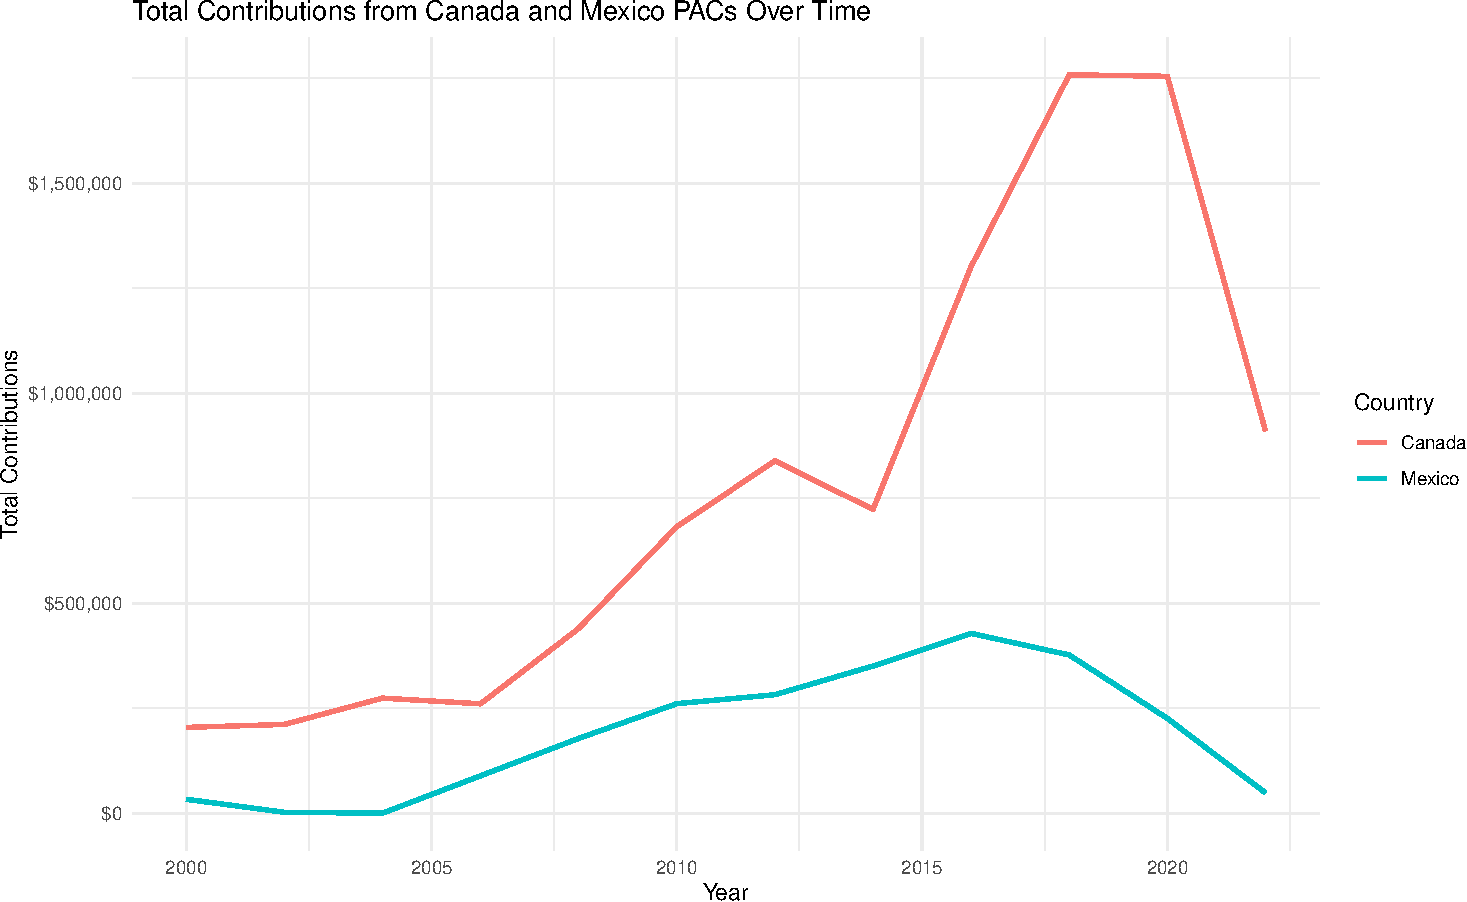
\includegraphics[width=0.8\linewidth]{hw-06-money-in-politics_files/figure-latex/canada-mexico-plot-1}

The plot shows that contributions from Canadian PACs have generally been
higher than those from Mexican PACs over most years. Both countries show
variability in their contribution patterns, with some years showing
significant spikes in contributions.

\begin{verbatim}
**Note:** The figure you create might look slightly different than this one if the data on the website has been updated recently.
\end{verbatim}

\begin{enumerate}
\def\labelenumi{\arabic{enumi}.}
\setcounter{enumi}{3}
\tightlist
\item
  Recreate the following visualisation. Once you have made the plot,
  write a brief interpretation of what the graph reveals. Note that
  these are only UK contributions. You will need to make use of
  functions from the \textbf{scales} package for axis labels as well as
  from \textbf{ggplot2}.
\end{enumerate}

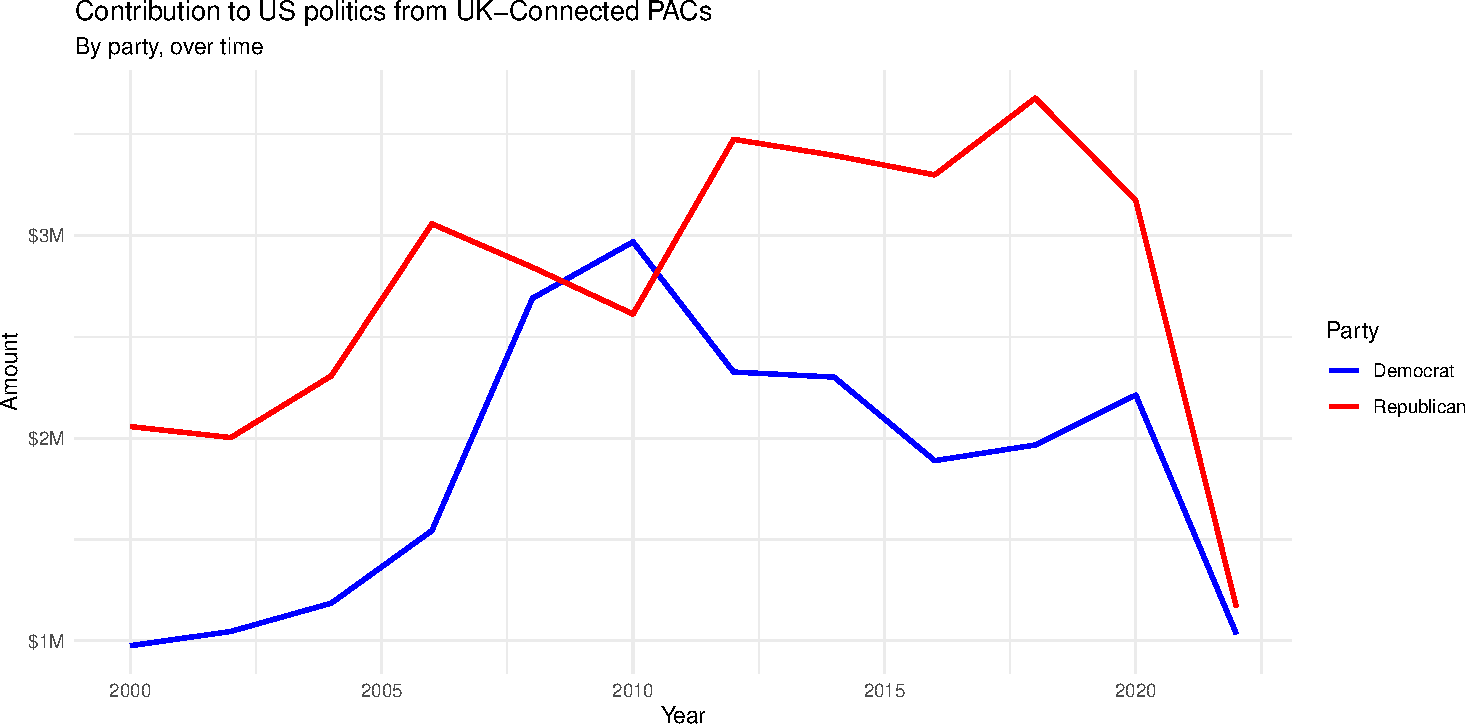
\includegraphics[width=0.8\linewidth]{hw-06-money-in-politics_files/figure-latex/unnamed-chunk-2-1}

\begin{Shaded}
\begin{Highlighting}[]
\CommentTok{\# Create UK contributions by party plot}
\NormalTok{pac\_all }\SpecialCharTok{\%\textgreater{}\%}
  \FunctionTok{separate}\NormalTok{(country\_parent, }\AttributeTok{into =} \FunctionTok{c}\NormalTok{(}\StringTok{"country"}\NormalTok{, }\StringTok{"parent"}\NormalTok{), }\AttributeTok{sep =} \StringTok{"/"}\NormalTok{, }\AttributeTok{extra =} \StringTok{"merge"}\NormalTok{) }\SpecialCharTok{\%\textgreater{}\%}
  \FunctionTok{mutate}\NormalTok{(}
    \AttributeTok{total =} \FunctionTok{str\_remove\_all}\NormalTok{(total, }\StringTok{"}\SpecialCharTok{\textbackslash{}\textbackslash{}}\StringTok{$|,"}\NormalTok{) }\SpecialCharTok{\%\textgreater{}\%} \FunctionTok{as.numeric}\NormalTok{(),}
    \AttributeTok{dems =} \FunctionTok{str\_remove\_all}\NormalTok{(dems, }\StringTok{"}\SpecialCharTok{\textbackslash{}\textbackslash{}}\StringTok{$|,"}\NormalTok{) }\SpecialCharTok{\%\textgreater{}\%} \FunctionTok{as.numeric}\NormalTok{(),}
    \AttributeTok{repubs =} \FunctionTok{str\_remove\_all}\NormalTok{(repubs, }\StringTok{"}\SpecialCharTok{\textbackslash{}\textbackslash{}}\StringTok{$|,"}\NormalTok{) }\SpecialCharTok{\%\textgreater{}\%} \FunctionTok{as.numeric}\NormalTok{()}
\NormalTok{  ) }\SpecialCharTok{\%\textgreater{}\%}
  \FunctionTok{filter}\NormalTok{(country }\SpecialCharTok{==} \StringTok{"UK"}\NormalTok{) }\SpecialCharTok{\%\textgreater{}\%}
  \FunctionTok{group\_by}\NormalTok{(year) }\SpecialCharTok{\%\textgreater{}\%}
  \FunctionTok{summarise}\NormalTok{(}
    \AttributeTok{Democrat =} \FunctionTok{sum}\NormalTok{(dems, }\AttributeTok{na.rm =} \ConstantTok{TRUE}\NormalTok{),}
    \AttributeTok{Republican =} \FunctionTok{sum}\NormalTok{(repubs, }\AttributeTok{na.rm =} \ConstantTok{TRUE}\NormalTok{),}
    \AttributeTok{.groups =} \StringTok{"drop"}
\NormalTok{  ) }\SpecialCharTok{\%\textgreater{}\%}
  \FunctionTok{pivot\_longer}\NormalTok{(}
    \AttributeTok{cols =} \FunctionTok{c}\NormalTok{(Democrat, Republican),}
    \AttributeTok{names\_to =} \StringTok{"party"}\NormalTok{,}
    \AttributeTok{values\_to =} \StringTok{"amount"}
\NormalTok{  ) }\SpecialCharTok{\%\textgreater{}\%}
  \FunctionTok{ggplot}\NormalTok{(}\FunctionTok{aes}\NormalTok{(}\AttributeTok{x =}\NormalTok{ year, }\AttributeTok{y =}\NormalTok{ amount, }\AttributeTok{color =}\NormalTok{ party)) }\SpecialCharTok{+}
  \FunctionTok{geom\_line}\NormalTok{(}\AttributeTok{size =} \DecValTok{1}\NormalTok{) }\SpecialCharTok{+}
  \FunctionTok{scale\_color\_manual}\NormalTok{(}\AttributeTok{values =} \FunctionTok{c}\NormalTok{(}\StringTok{"Democrat"} \OtherTok{=} \StringTok{"blue"}\NormalTok{, }\StringTok{"Republican"} \OtherTok{=} \StringTok{"red"}\NormalTok{)) }\SpecialCharTok{+}
  \FunctionTok{scale\_y\_continuous}\NormalTok{(}\AttributeTok{labels =} \FunctionTok{dollar\_format}\NormalTok{(}\AttributeTok{scale =} \FloatTok{0.000001}\NormalTok{, }\AttributeTok{suffix =} \StringTok{"M"}\NormalTok{)) }\SpecialCharTok{+}
  \FunctionTok{labs}\NormalTok{(}
    \AttributeTok{x =} \StringTok{"Year"}\NormalTok{,}
    \AttributeTok{y =} \StringTok{"Amount"}\NormalTok{,}
    \AttributeTok{color =} \StringTok{"Party"}\NormalTok{,}
    \AttributeTok{title =} \StringTok{"Contribution to US politics from UK{-}Connected PACs"}\NormalTok{,}
    \AttributeTok{subtitle =} \StringTok{"By party, over time"}
\NormalTok{  ) }\SpecialCharTok{+}
  \FunctionTok{theme\_minimal}\NormalTok{()}
\end{Highlighting}
\end{Shaded}

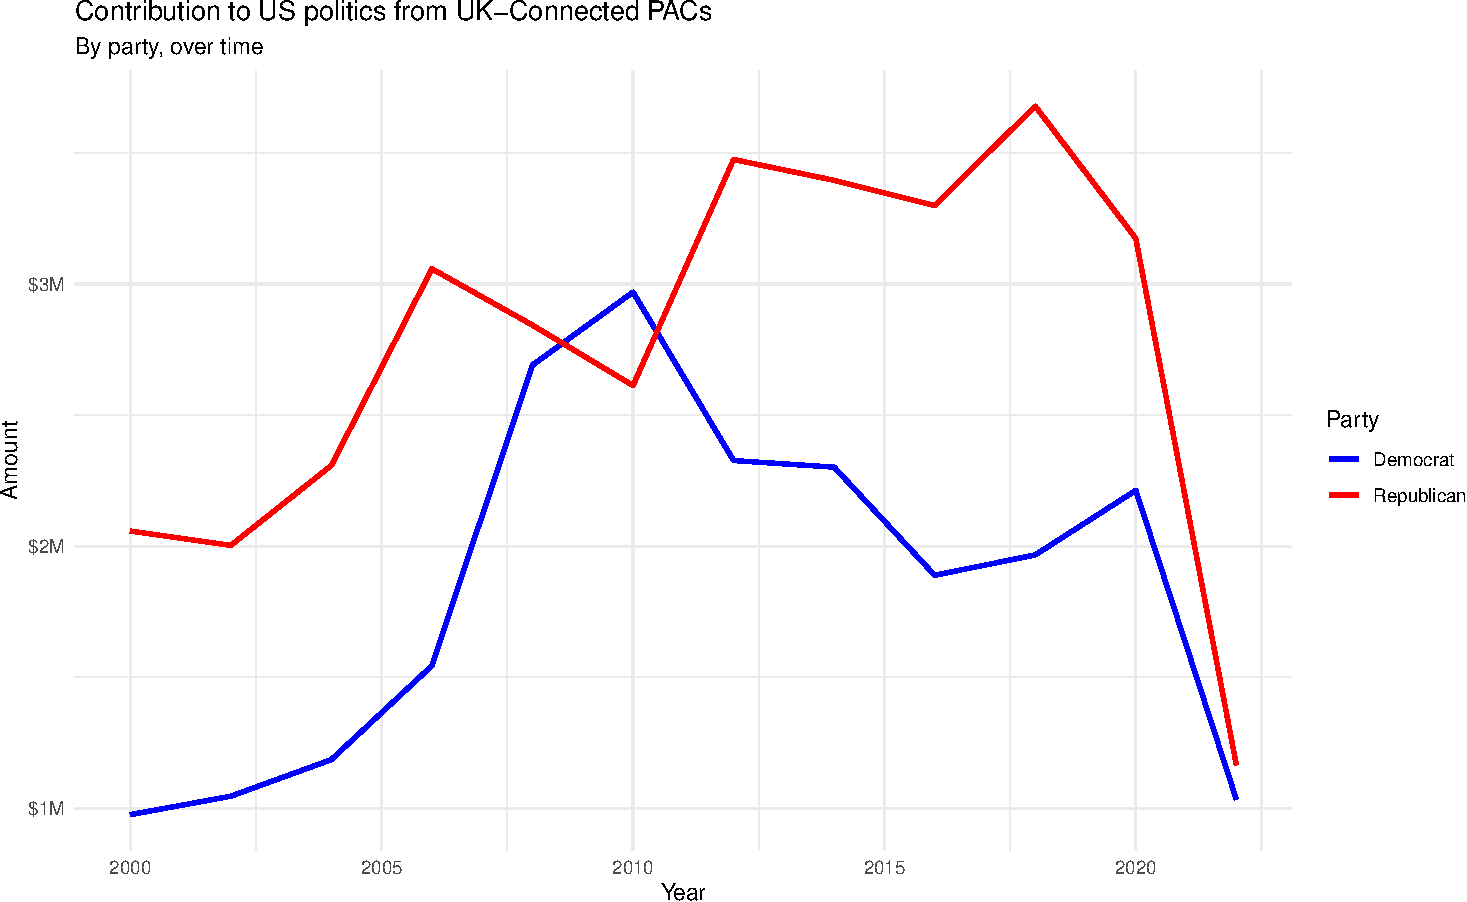
\includegraphics[width=0.8\linewidth]{hw-06-money-in-politics_files/figure-latex/uk-party-contributions-1}

The plot reveals that UK-connected PACs have generally contributed more
to Republican candidates than Democratic candidates over most election
cycles. There are notable fluctuations in both parties' contributions
over time, with some years showing particularly high contributions to
one party or the other.

Knit, \emph{commit, and push your changes to GitHub with an appropriate
commit message. Make sure to commit and push all changed files so that
your Git pane is cleared up afterwards and review the md document on
GitHub to make sure you're happy with the final state of your work.}

\end{document}
